%!TEX TS-program = xelatex

% Официальный шаблон презентации НИУ ВШЭ в beamer (LaTeX)
% Версия 2.0
% Язык — русский

\documentclass[aspectratio=169]{beamer}

\newbool{russian}
\booltrue{russian}
\usepackage{HSE-theme/beamerthemeHSE}

%%% Работа с русским языком и шрифтами
\usepackage{multirow}
\usepackage{listings} 
\usepackage[dvipsnames]{xcolor}
\usepackage[english,russian]{babel}
\usepackage[no-math]{fontspec}
\usepackage{makecell}
	\IfFontExistsTF{HSE Sans}
		{\newcommand{\presentationfont}{HSE Sans}}
		{\newcommand{\presentationfont}{Arial}}
	\setsansfont{\presentationfont}
	\setmonofont{Courier New}

\usepackage[most]{tcolorbox}

\usepackage{mathspec}
	\setmathsfont(Digits,Latin,Greek)[Numbers={Lining,Proportional}]{\presentationfont}
	\setmathrm[Numbers={Lining,Proportional}]{\presentationfont}
\uselanguage{russian}
\languagepath{russian}
\deftranslation[to=russian]{Theorem}{Теорема}
\deftranslation[to=russian]{Definition}{Определение}
\deftranslation[to=russian]{Definitions}{Определения}
\deftranslation[to=russian]{Corollary}{Следствие}
\deftranslation[to=russian]{Fact}{Факт}
\deftranslation[to=russian]{Example}{Пример}
\deftranslation[to=russian]{Examples}{Примеры}

\usepackage{booktabs}
\usepackage{array}
\graphicspath{{images/}}


\newcommand{\term}[1]{{\large\textcolor{HSEblue}{#1}}}
\newcommand{\cmd}[1]{\textcolor{HSEblue}{\texttt{#1}}}
\newcommand{\todo}[1]{\textcolor{red}{[TODO: #1]}}

\newenvironment{demoblock}[1]
	{\begin{exampleblock}{Демо: #1}\small}
	{\end{exampleblock}}

\lstset{ 
    basicstyle=\color{HSEblue}\ttfamily\small,
    numbers=left,
    numberstyle=\color{HSEblue}\ttfamily\scriptsize,
    frame=single,
    columns=fullflexible,
    keepspaces=true,
    showstringspaces=false,
    breaklines=true,
    rulecolor=\color{HSEblue},
}


%% Информация об авторе и выступлении

\title[Мобильные колесные роботы]{Математическая модель мобильного робота и ROS2}
\subtitle{Проектный семинар <<Мобильные колесные роботы>>}
\author[Команда курса]{Дергачев Степан  Алексеевич, \texttt{\href{mailto:sadergachev@hse.ru}{sadergachev@hse.ru}} \\ Муравьев Кирилл Федорович, \texttt{\href{mailto:kmuravev@hse.ru}{kmuravev@hse.ru}}}
\institute{Факультет компьютерных наук НИУ ВШЭ}
\date{08 октября 2026}

\begin{document}

\frame[plain]{\titlepage}

\section{Модель движения как динамическая система}

\begin{frame}
\frametitle{Математическая модель мобильного робота}
\begin{columns}[T]
\column{0.65\textwidth}
\small
\begin{itemize}
  \item Модель описывает движение робота и позволяет прогнозировать его состояние, выбирать управление и оценивать перемещение.
  \item Вектор состояния робота $\mathbf x$ включает в себя набор величин, которые описывают его положение в пространстве и внутреннюю конфигурацию. Например: $\mathbf x = (p_x,p_y,\theta)$.
  \item Вектор управления $\mathbf u$ -- это набор величин, которые подаются на исполнительные механизмы робота для изменения его состояния. Например: $\mathbf u=(v,w)$.
\end{itemize}
\column{0.32\textwidth}
\vfill
	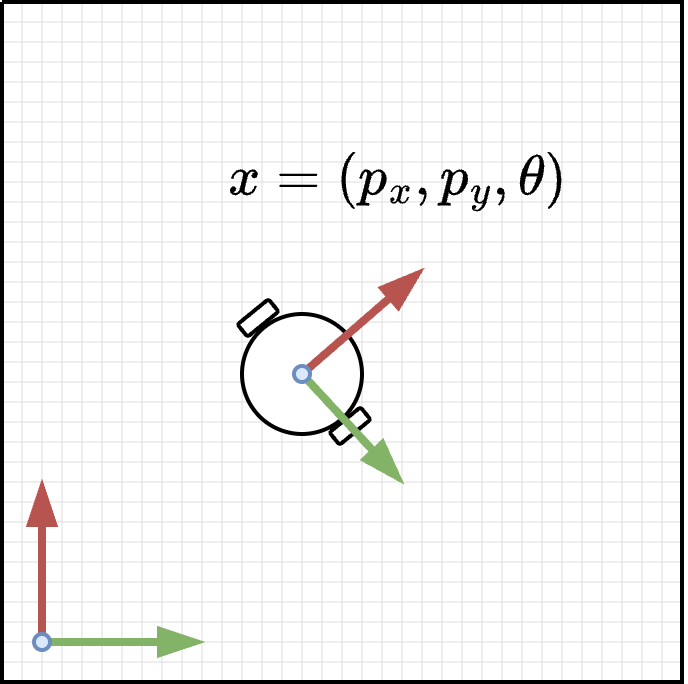
\includegraphics[width=0.99\columnwidth]{images/axis.png}
  \vfill
\end{columns}
\end{frame}

\begin{frame}
\frametitle{Математическая модель мобильного робота}
\begin{columns}[T]
\column{0.65\textwidth}
\small
\begin{itemize}
  \item Для описания состояния робота (обычно) используется неподвижная мировая система координат. 
  
  \item Выделяют систему координат корпуса робота, которая движется вместе с роботом. 
  
  \item Составные части робота (в том числе датчики) могут обладать своими системами координат.
\end{itemize}
\column{0.32\textwidth}
\vfill
	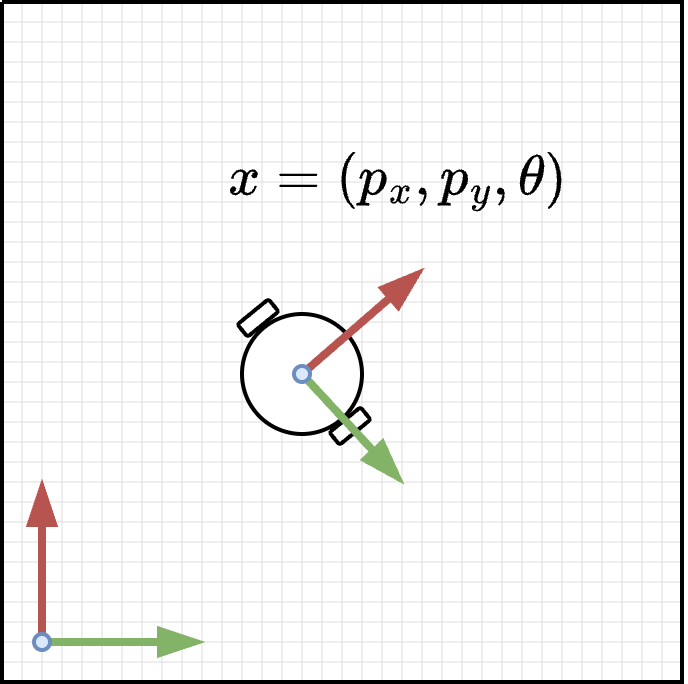
\includegraphics[width=0.99\columnwidth]{images/axis.png}
  \vfill
\end{columns}
\end{frame}

\begin{frame}
\frametitle{Прямая и обратная задача кинематики}
\begin{columns}[T]
\column{0.47\textwidth}
\begin{block}{Прямая задача кинематики}
\begin{itemize}
  \item По управлению определить изменение состояния робота.
\end{itemize}
\end{block}
\column{0.47\textwidth}
\begin{block}{Обратная задача кинематики}
\begin{itemize}
  \item По требуемому изменению состояния и заданному времени определить необходимое управление.
\end{itemize}
\end{block}
\end{columns}
\vfill
\begin{columns}[T]
\column{0.49\textwidth}
\centering
\vfill
	
\includegraphics[height=1.5cm]{images/fwd_kin.png}
  \vfill
\column{0.49\textwidth}
\centering
\vfill
	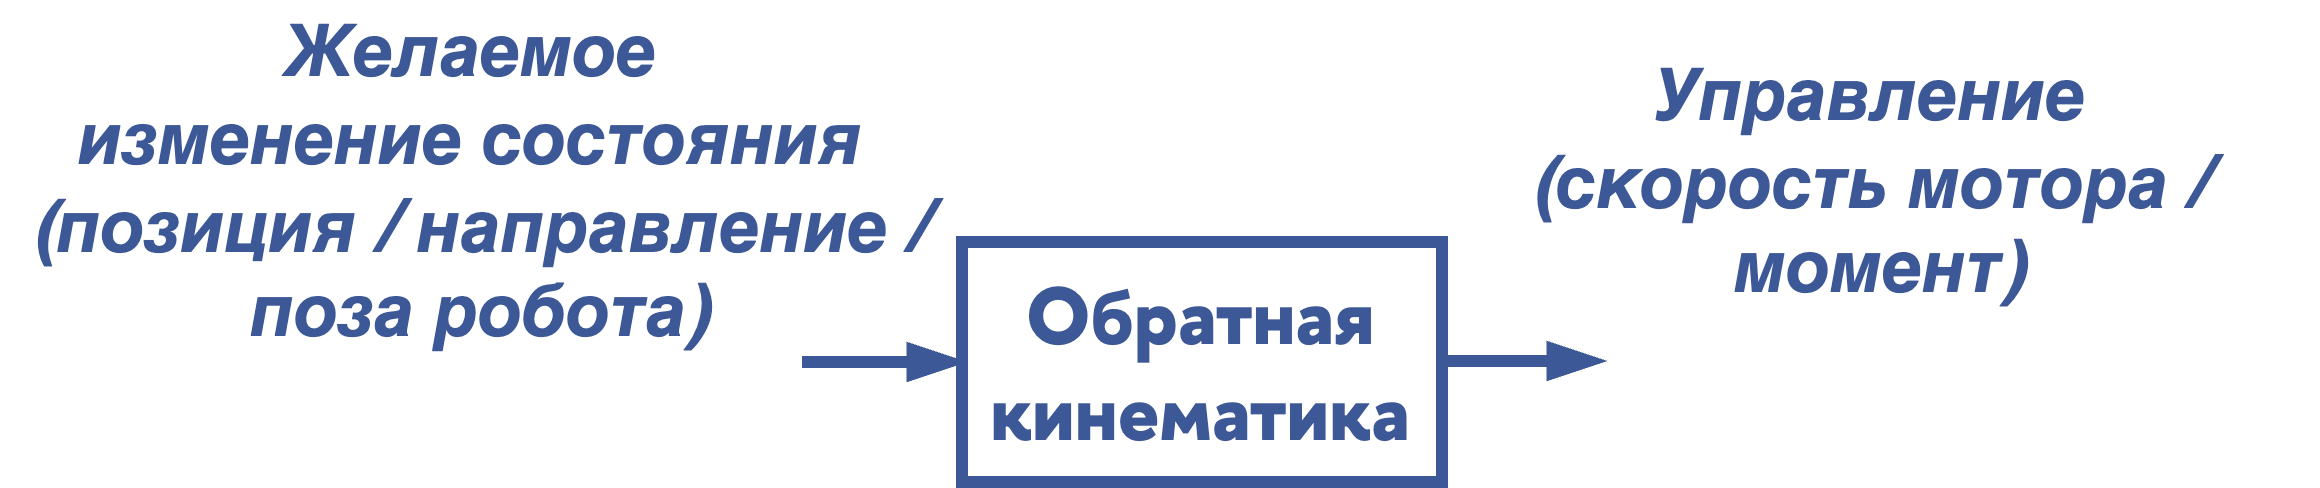
\includegraphics[height=1.5cm]{images/inv_kin.png}
  \vfill
\end{columns}


\end{frame}

\begin{frame}
\frametitle{Модель мобильного робота как динамическая система}
\small
\begin{block}{Непрерывная модель}
  \begin{itemize}
  \item Состояние и управление определены в каждый момент времени. Модель задает изменение состояния:
  \end{itemize}
\[
  \dot{\mathbf x}=f(\mathbf x(t),\mathbf u(t)),
\]
\end{block}
\vfill
\begin{block}{Дискретная модель}
  \begin{itemize}
  \item Состояние рассматривается в отдельные моменты времени $t$. Модель задает переход от состояния к состоянию:
  \end{itemize}
\[
  \mathbf x_{t+1}=F(\mathbf x_t,\mathbf u_t),
\]
\end{block}
Модель робота также может включать:  модель выхода системы $\mathbf y$ (например, модель показаний датчиков в зависимости от состояния и управления), ограничения на состояние и управление, неточности параметров и случайные возмущения.

\end{frame}

\begin{frame}
\frametitle{Ограничения}
\renewcommand{\arraystretch}{1.2}
\small
\begin{tabular}{>{\raggedright\arraybackslash}m{0.23\textwidth}>{\raggedright\arraybackslash}m{0.68\textwidth}}
\toprule
\term{Тип} & \term{Что ограничивают} \\
\midrule
Геометрические & Допустимые положения элементов системы\\
Кинематические & Допустимые скорости движения элементов системы \\
Динамические & Ограничения возможных ускорений системы, сил, моментов приводов и т.д. \\
\bottomrule
\end{tabular}
\vfill
\begin{block}{Примеры явных ограничений}
\begin{itemize}
  \item  $\|v\|\leq v_{\max}$, $\|w\|\leq w_{\max}$ -- ограничения на максимальные скорости
  \item  $\|\dot v\|\leq a_{\max}$ -- ограничение на максимальное ускорение 
\end{itemize}

\end{block}
\end{frame}

\begin{frame}
\frametitle{Неопределенность в модели}
\begin{block}{Шум изменения состояния}
\[
 \mathbf x_{t+1}=F(\mathbf x_t,\mathbf u_t)+\mathbf \varepsilon_t,
 \qquad \mathbf \varepsilon_t\sim\mathcal N( 0, \Sigma_t)
\]
\small
Описывает ошибку шага модели. Позволяет учитывать разные причины, но параметры шума сложнее связать с физикой движения.
\end{block}
\begin{block}{Шум управления}
\[
 \mathbf x_{t+1}=F(\mathbf x_t,\mathbf u_t+\varepsilon_t),
 \qquad \varepsilon_t\sim\mathcal N(0, \Sigma_t)
\]
\small
Описывает ошибки исполнения управления. Их влияние на позу зависит от кинематики.
\end{block}
\vfill
\scriptsize
\rule[0.5ex]{0.3\linewidth}{0.1pt}\\
\textit{$^*$ Нормальное распределение -- допущение модели, могут использоваться другие распределения.}
\end{frame}

\section{Модели движения колесных роботов}

\begin{frame}
\frametitle{Виды колесных платформ}
\begin{columns}[T]
\column{0.47\textwidth}   

   
\begingroup
\setlength{\fboxrule}{0.4pt} % Толщина обводки
\setlength{\fboxsep}{6pt}   % Внутренний отступ
\noindent
\fcolorbox{HSEblue}{white}{%
  \begin{minipage}{\dimexpr\linewidth-2\fboxsep-2\fboxrule\relax}
    \begin{block}{Дифференциальный привод}
      \small
      Независимое вращение левого и правого колес.
\begin{center}
    	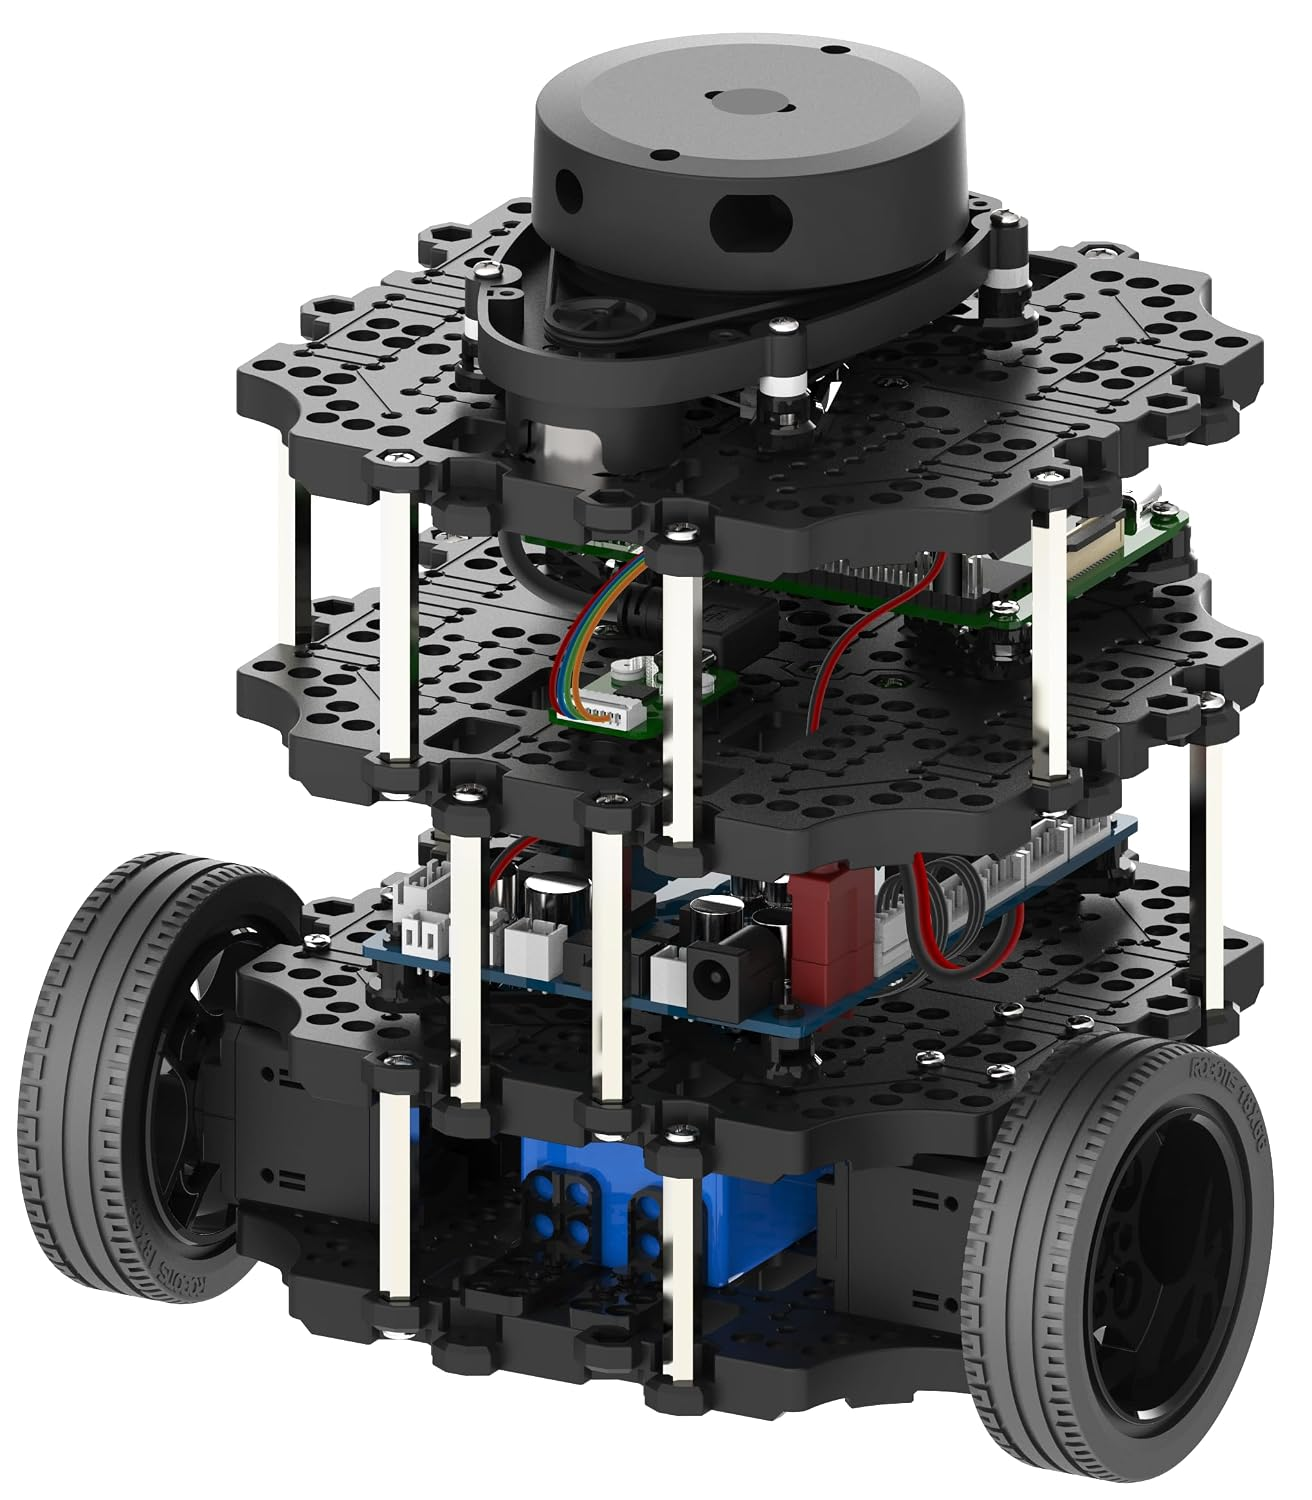
\includegraphics[height=1.5cm]{images/turtlebot3.jpg}
\end{center}
    \end{block}
  \end{minipage}%
}
\endgroup

\begin{block}{Omni-колеса}
\small
Свободные ролики на колесе позволяют двигаться боком.
\begin{center}
  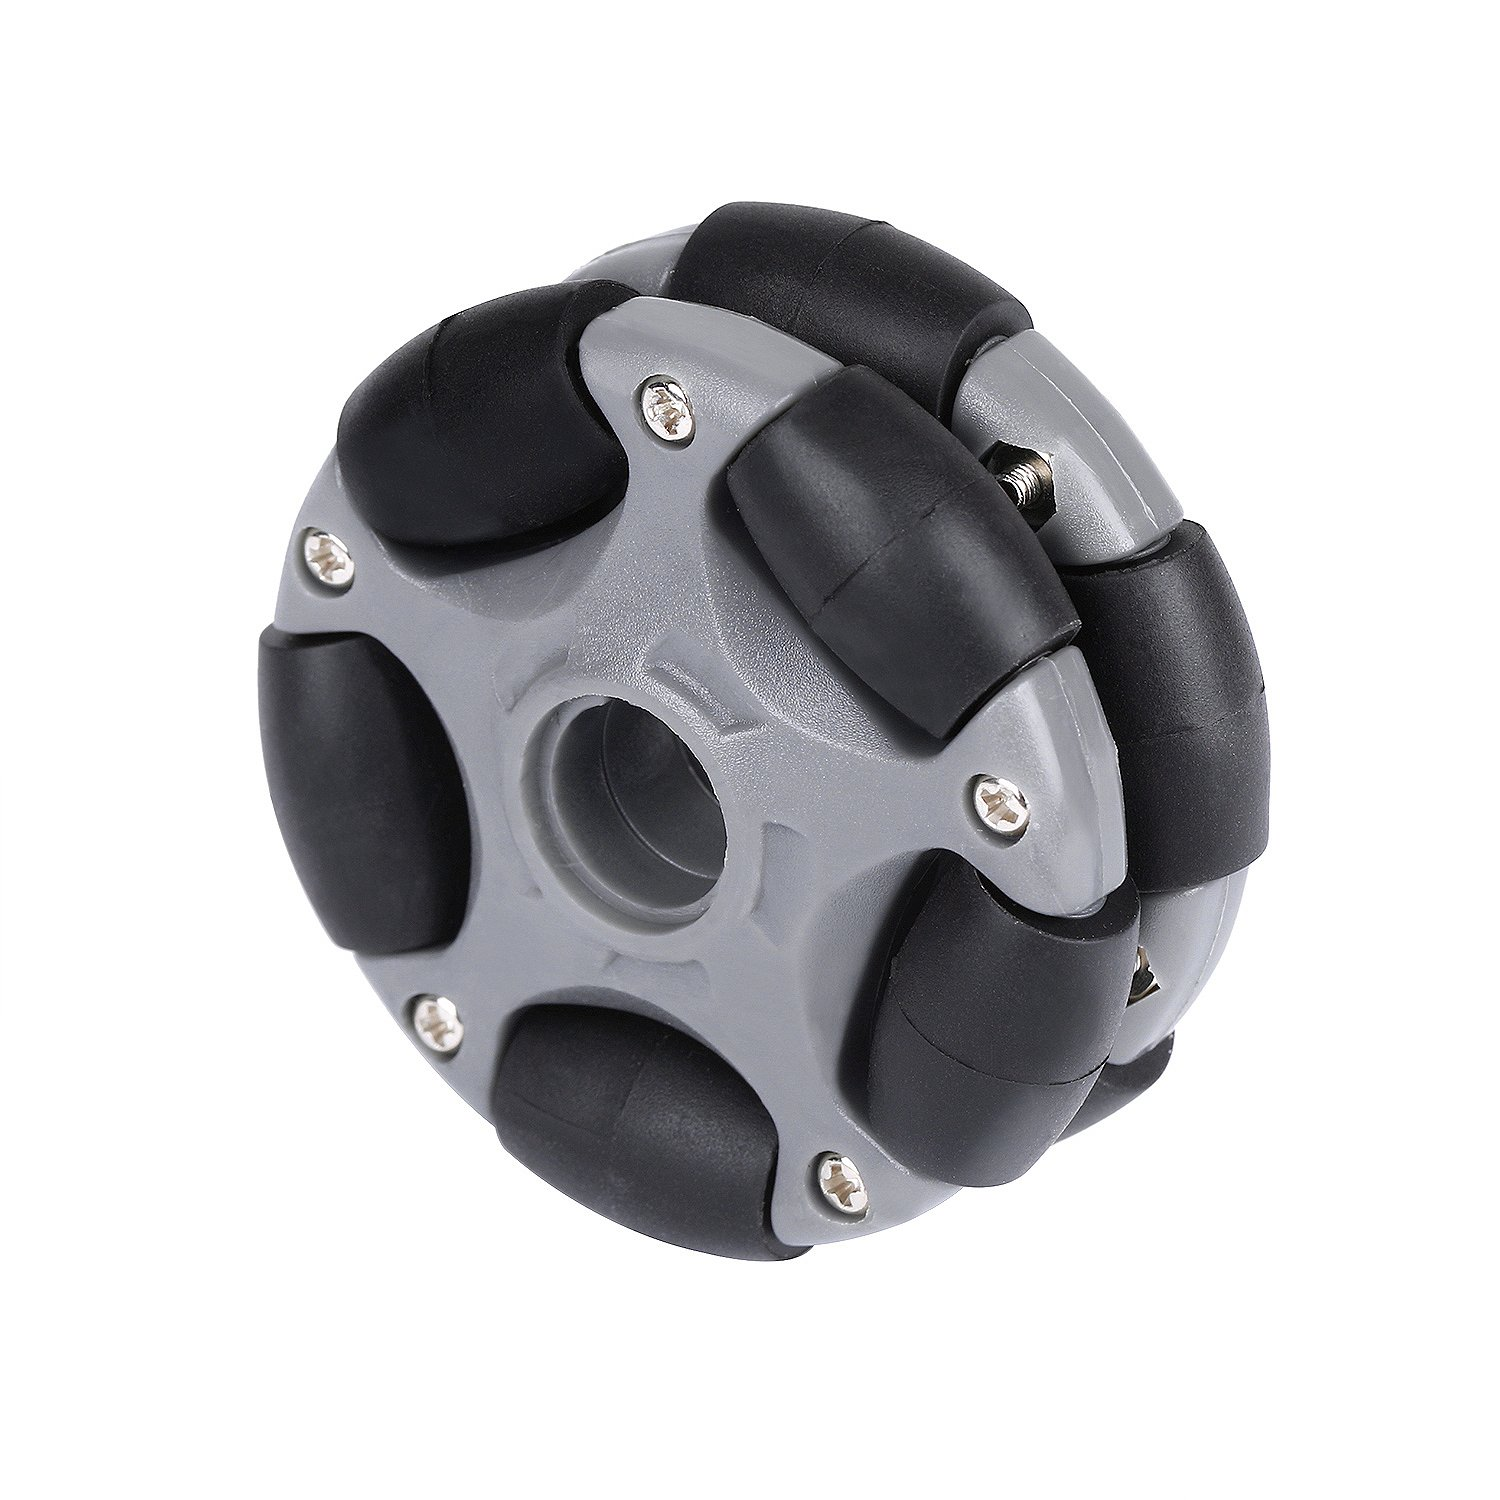
\includegraphics[height=1.5cm]{images/omni.jpg}\hspace{0.5 cm}
  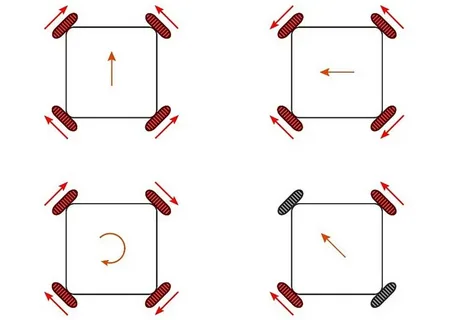
\includegraphics[height=1.5cm]{images/omni_ctrl.png}
\end{center}
\end{block}
\column{0.47\textwidth}
\begin{block}{Автомобильная платформа}
\small
Поворот за счет руления. Есть минимальный радиус поворота.
\begin{center}
  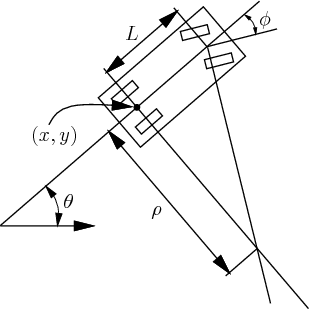
\includegraphics[height=1.5cm]{images/car.png}
\end{center}
\end{block}
\begin{block}{Колеса Mecanum}
\small
Наклонные ролики на колесе позволяют двигаться боком
\begin{center}
  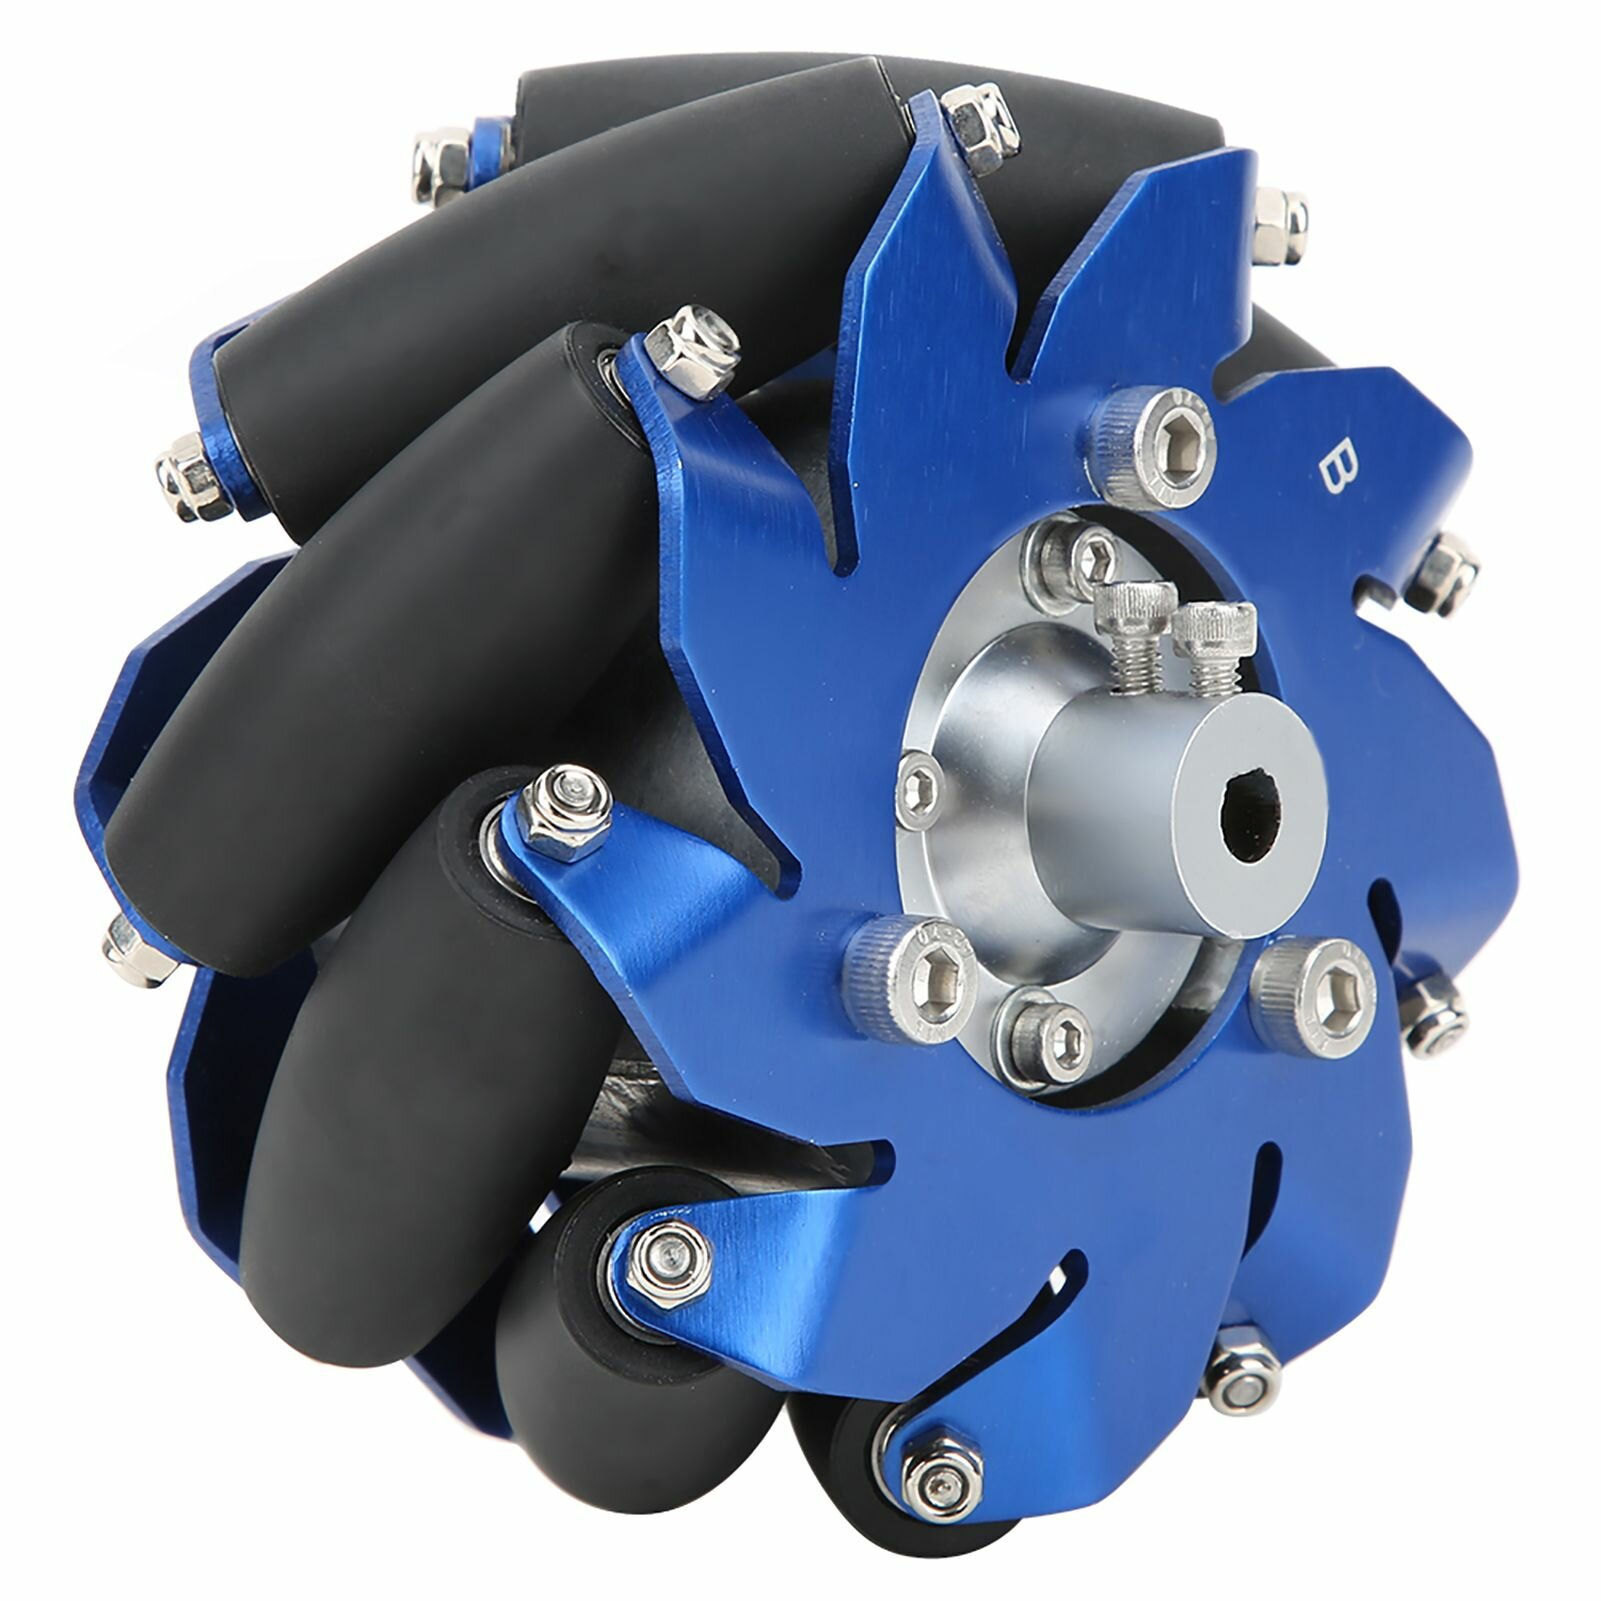
\includegraphics[height=1.5cm]{images/mecanum.jpg}\hspace{0.5 cm}
  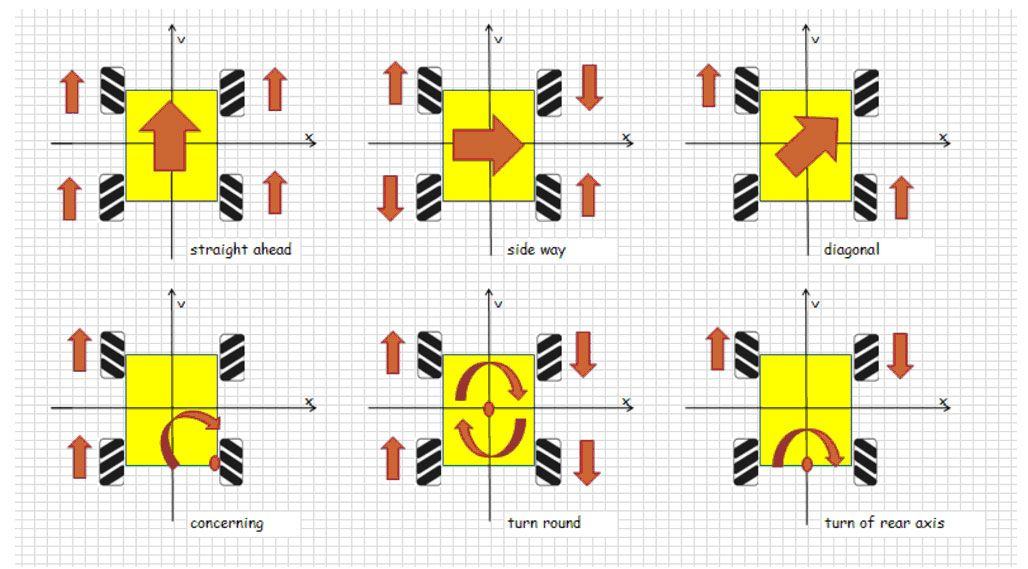
\includegraphics[height=1.5cm]{images/mecanum_ctrl.jpg}
\end{center}
\end{block}
\end{columns}
\end{frame}

\begin{frame}
\frametitle{Модель Single Integrator}
\begin{columns}[T]
\column{0.60\textwidth}
\begin{itemize}
  \item Состояние -- позиция $\mathbf x=(p_x,p_y)$.
  \item Управление -- скорость в мировой системе координат: $\mathbf u=(v_x,v_y)$.
  \item Направление скорости может меняться мгновенно.
\end{itemize}
\[
 \mathbf x_{t+1}=\mathbf x_t+\mathbf u_t\Delta t \qquad \|\mathbf u\|\leq v_{\max}
\]
\column{0.36\textwidth}
\vfill
  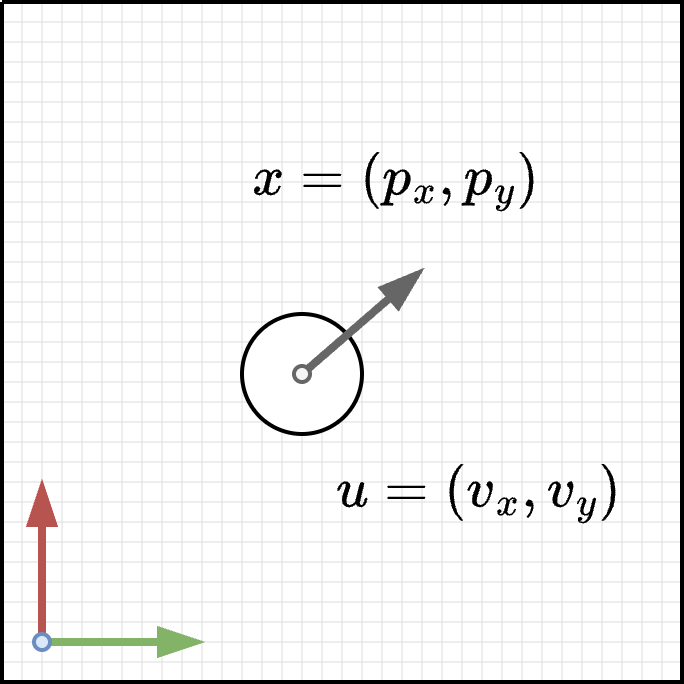
\includegraphics[width=\columnwidth]{images/si.png}
\vfill
\end{columns}
\vfill
Удобная абстракция для планирования, но не учитывает многих ограничений колесной платформы (ускорение, невозможность движения "боком" и т.д.).
\end{frame}

\begin{frame}
\frametitle{Модель Double Integrator}
\begin{columns}[T]
\column{0.6\textwidth}
\begin{itemize}
  \item Состояние -- положение и скорость: $\mathbf x=(p_x, p_y, v_x, v_y)$.
  \item Управление -- ускорение $\mathbf u=(a_x,a_y)$ в мировой системе координат.
\end{itemize}
\[
 \begin{aligned}
 \mathbf x_{t+1}&=\mathbf x_t+\mathbf v_t \Delta t+\tfrac12\mathbf u_t \Delta t^2,\\
 \mathbf v_{t+1}&=\mathbf v_t+\mathbf u_t \Delta t
 \end{aligned}
\]
\[
 \|\mathbf u_t\|\leq a_{\max},\qquad \|\mathbf v_t\|\leq v_{\max}
\]
\column{0.36\textwidth}
\vfill
  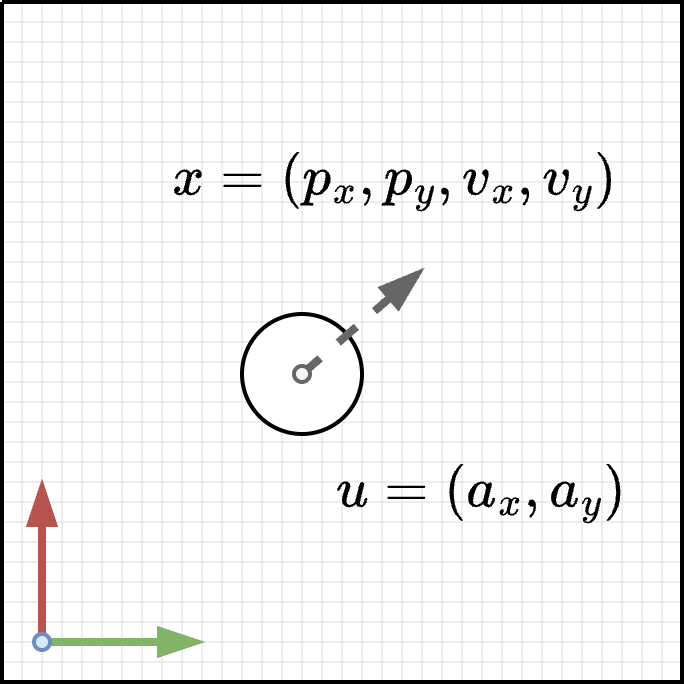
\includegraphics[width=\columnwidth]{images/di.png}
\vfill
\end{columns}
\vfill
Учитывает ограничение на ускорение, но не описывает невозможность движения "боком".
\end{frame}

\begin{frame}
\frametitle{Модель Differential-drive}
\begin{columns}[T]
\column{0.6\textwidth}
\small
\begin{itemize}
  \item Два независимо приводимых в движение колеса радиуса $r$. Расстояние между колесами $L$.
  \item Состояние робота задается позицией середины оси колес и направлением $\mathbf x = (p_x, p_y, \theta)$ .
  \item Предполагается, что колеса движутся без продольного и бокового проскальзывания. Боковая скорость всегда равна нулю.
  \item Движение задается изменением угловых скоростей колес $w_L$, $w_R$. Можно вычислить продольные скорости $v_L$, $v_R$ центров колес:
  \[
  v_L = r\cdot w_L,\quad v_R = r\cdot w_R
  \]
\end{itemize}
\column{0.35\textwidth}
% \small
% \begin{itemize}
%   \item $w_L=w_R$: прямая.
%   \item $w_L \ne w_R$: дуга.
%   \item $w_L=-w_R\ne0$: вращение на месте.
% \end{itemize}
\vfill
\begin{center}
    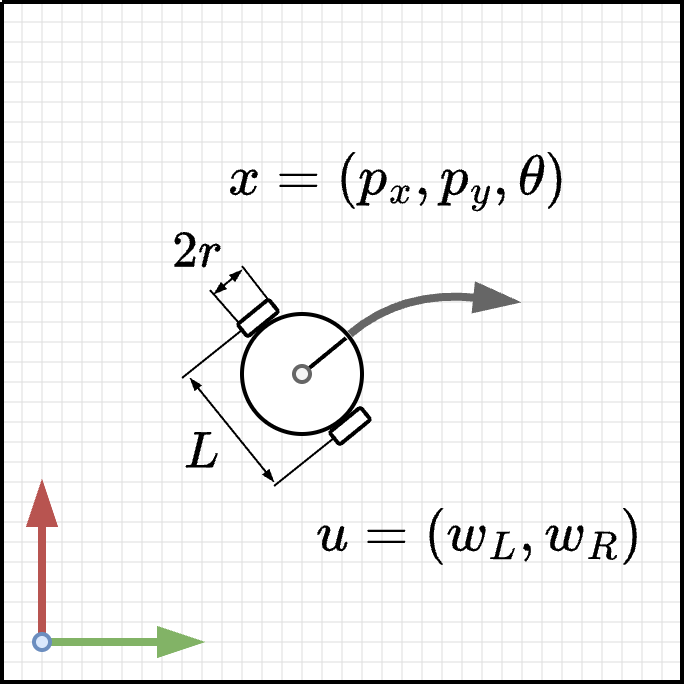
\includegraphics[width=\columnwidth]{images/dd_wh.png}
\end{center}
\vfill
\end{columns}
\end{frame}

\begin{frame}
\frametitle{Модель Differential-drive}
\begin{columns}[T]
\column{0.6\textwidth}
\begin{itemize}
  \item Удобнее использовать для управления линейную и угловую скорости корпуса:

\[
 v =\frac{(v_R+v_L)}{2},\qquad
 w =\frac{(v_R-v_L)}{L}
\]
\item Непрерывная модель:
\[
 \begin{cases}
 \dot x = v \cos{\theta},\\
 \dot y = v \sin{\theta},\\
 \dot{\theta}= w
 \end{cases}
\]
\end{itemize}
\column{0.35\textwidth}
% \small
% \begin{itemize}
%   \item $w_L=w_R$: прямая.
%   \item $w_L \ne w_R$: дуга.
%   \item $w_L=-w_R\ne0$: вращение на месте.
% \end{itemize}
\vfill
\begin{center}
    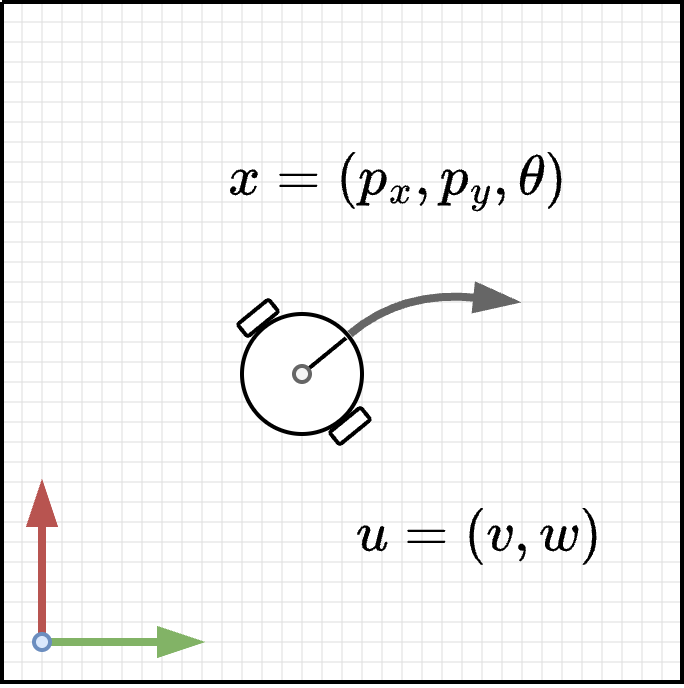
\includegraphics[width=\columnwidth]{images/dd_vel.png}
\end{center}
\vfill
\end{columns}
\end{frame}

\begin{frame}
\frametitle{Модель Differential-drive}
\begin{columns}[T]
\column{0.57\textwidth}
\small
\begin{block}{Дискретная модель: метод Эйлера}
\[
 \begin{cases}
 p_{x,k+1}=p_{x,k}+v_t\cos{\theta}_t \Delta t,\\
 p_{y,k+1}=p_{y,k}+v_t\sin{\theta}_t \Delta t,\\
 {\theta}_{t+1}={\theta}_t+w_t \Delta t
 \end{cases}
\]
\end{block}
\begin{block}{Дискретная модель: мгновенный центр вращения}
Более точное вычисление -- через мгновенный центр вращения (ICC):
\[
 R = \frac v w = \frac{L}{2}\cdot\frac{w_R+w_L}{w_R-w_L}
\]
\[
 (ICC_x,ICC_y)=(p_x-R\sin{\theta},\ p_y+R\cos{\theta})
\]

\end{block}
\column{0.39\textwidth}
\begin{center}
    \vfill
    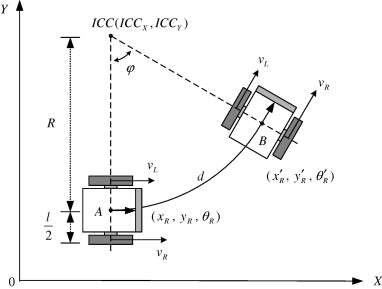
\includegraphics[width=\columnwidth]{images/icc.jpg}
    \vfill
\end{center}
\end{columns}
\end{frame}

\section{Оценка положения по модели}

\begin{frame}
\frametitle{Оценка перемещения: Одометрия}
\small
\term{Одометрия} -- оценка перемещения робота на основе данных о его движении
\vfill
\begin{itemize}
  \item Накопление приращений дает позу относительно начала движения
  \item Одометрия $\ne$ локализация. 
\end{itemize}
 \vfill
\renewcommand{\arraystretch}{1.10}
\begin{tabular}{>{\raggedright\arraybackslash}m{0.3\textwidth}>{\raggedright\arraybackslash}m{0.66\textwidth}}
\toprule
\textcolor{HSEblue}{Пример} & \textcolor{HSEblue}{Источник} \\
\midrule
Одометрия по управляющим сигналам & Заданные скорости и модель движения. \\
\textcolor{HSEblue}{\textbf{Колесная одометрия}} & Углы поворота или скорости колес по энкодерам. \\
Инерциальная одометрия & Ускорения и угловые скорости по IMU. \\
Визуальная одометрия & Изменение кадров в последовательности изображений с камеры. \\
Лидарная одометрия & Изменение лучей в последовательности сканов LiDAR. \\

\bottomrule
\end{tabular}
\vfill
\end{frame}


\begin{frame}
\frametitle{Ошибки одометрии}
\begin{itemize}
  \small
  \item Проскальзывание колес, неточно заданные параметры робота, шум датчиков приводят к небольшим ошибкам на каждом шаге.
  \item Небольшие ошибки со временем накапливаются.
\end{itemize}
\vfill
\renewcommand{\arraystretch}{1.1}
\small
\begin{tabular}{>{\raggedright\arraybackslash}m{0.23\textwidth}>{\raggedright\arraybackslash}m{0.68\textwidth}}
\toprule
\textcolor{HSEblue}{Источник} & \textcolor{HSEblue}{Ограничения} \\
\midrule
Управление & Точное исполнение команд невозможно, никак не учитываются проскальзования изастревания робота\\
Энкодеры & Измеряют вращение колес, но не обнаруживают проскальзывания. \\
IMU & Погрешности измерения угловых скоростей и ускорений очень быстро накапливаются при интегрировании. \\
Камеры & Сильная зависимость от текстуры, освещения и движения объектов в среде, вычислительная сложность \\
LiDAR & Сильная зависимость от наполнения среды, вычислительная сложность \\
\bottomrule
\end{tabular}
\end{frame}

\section{ROS 2, ros2\_control и tf2}

\begin{frame}[fragile]
\frametitle{Системы координат в ROS2}
\begin{columns}[T]
\column{0.60\textwidth}
\small
\begin{itemize}
  \item \cmd{tf2} -- библиотекав в ROS2, предназначенная для отслеживания, вычисления и хранения преобразований  между системами координат в виде дерева.
  \item Узел дерева (frame) - конкретная система координат. 
  \item Ребро дерева (transform) -- перенос и поворот дочерней системы относительно родительской.
  \item Направление осей: $OX$ вперед, $OY$ влево, $OZ$ вверх (правая система).
  \item Единицы измерения: метры и радианы.
  \item Поворот представляется кватернионом, но может задаваться через углы Эйлера.
\end{itemize}
\column{0.39\textwidth}
\begin{center}
    \vfill
    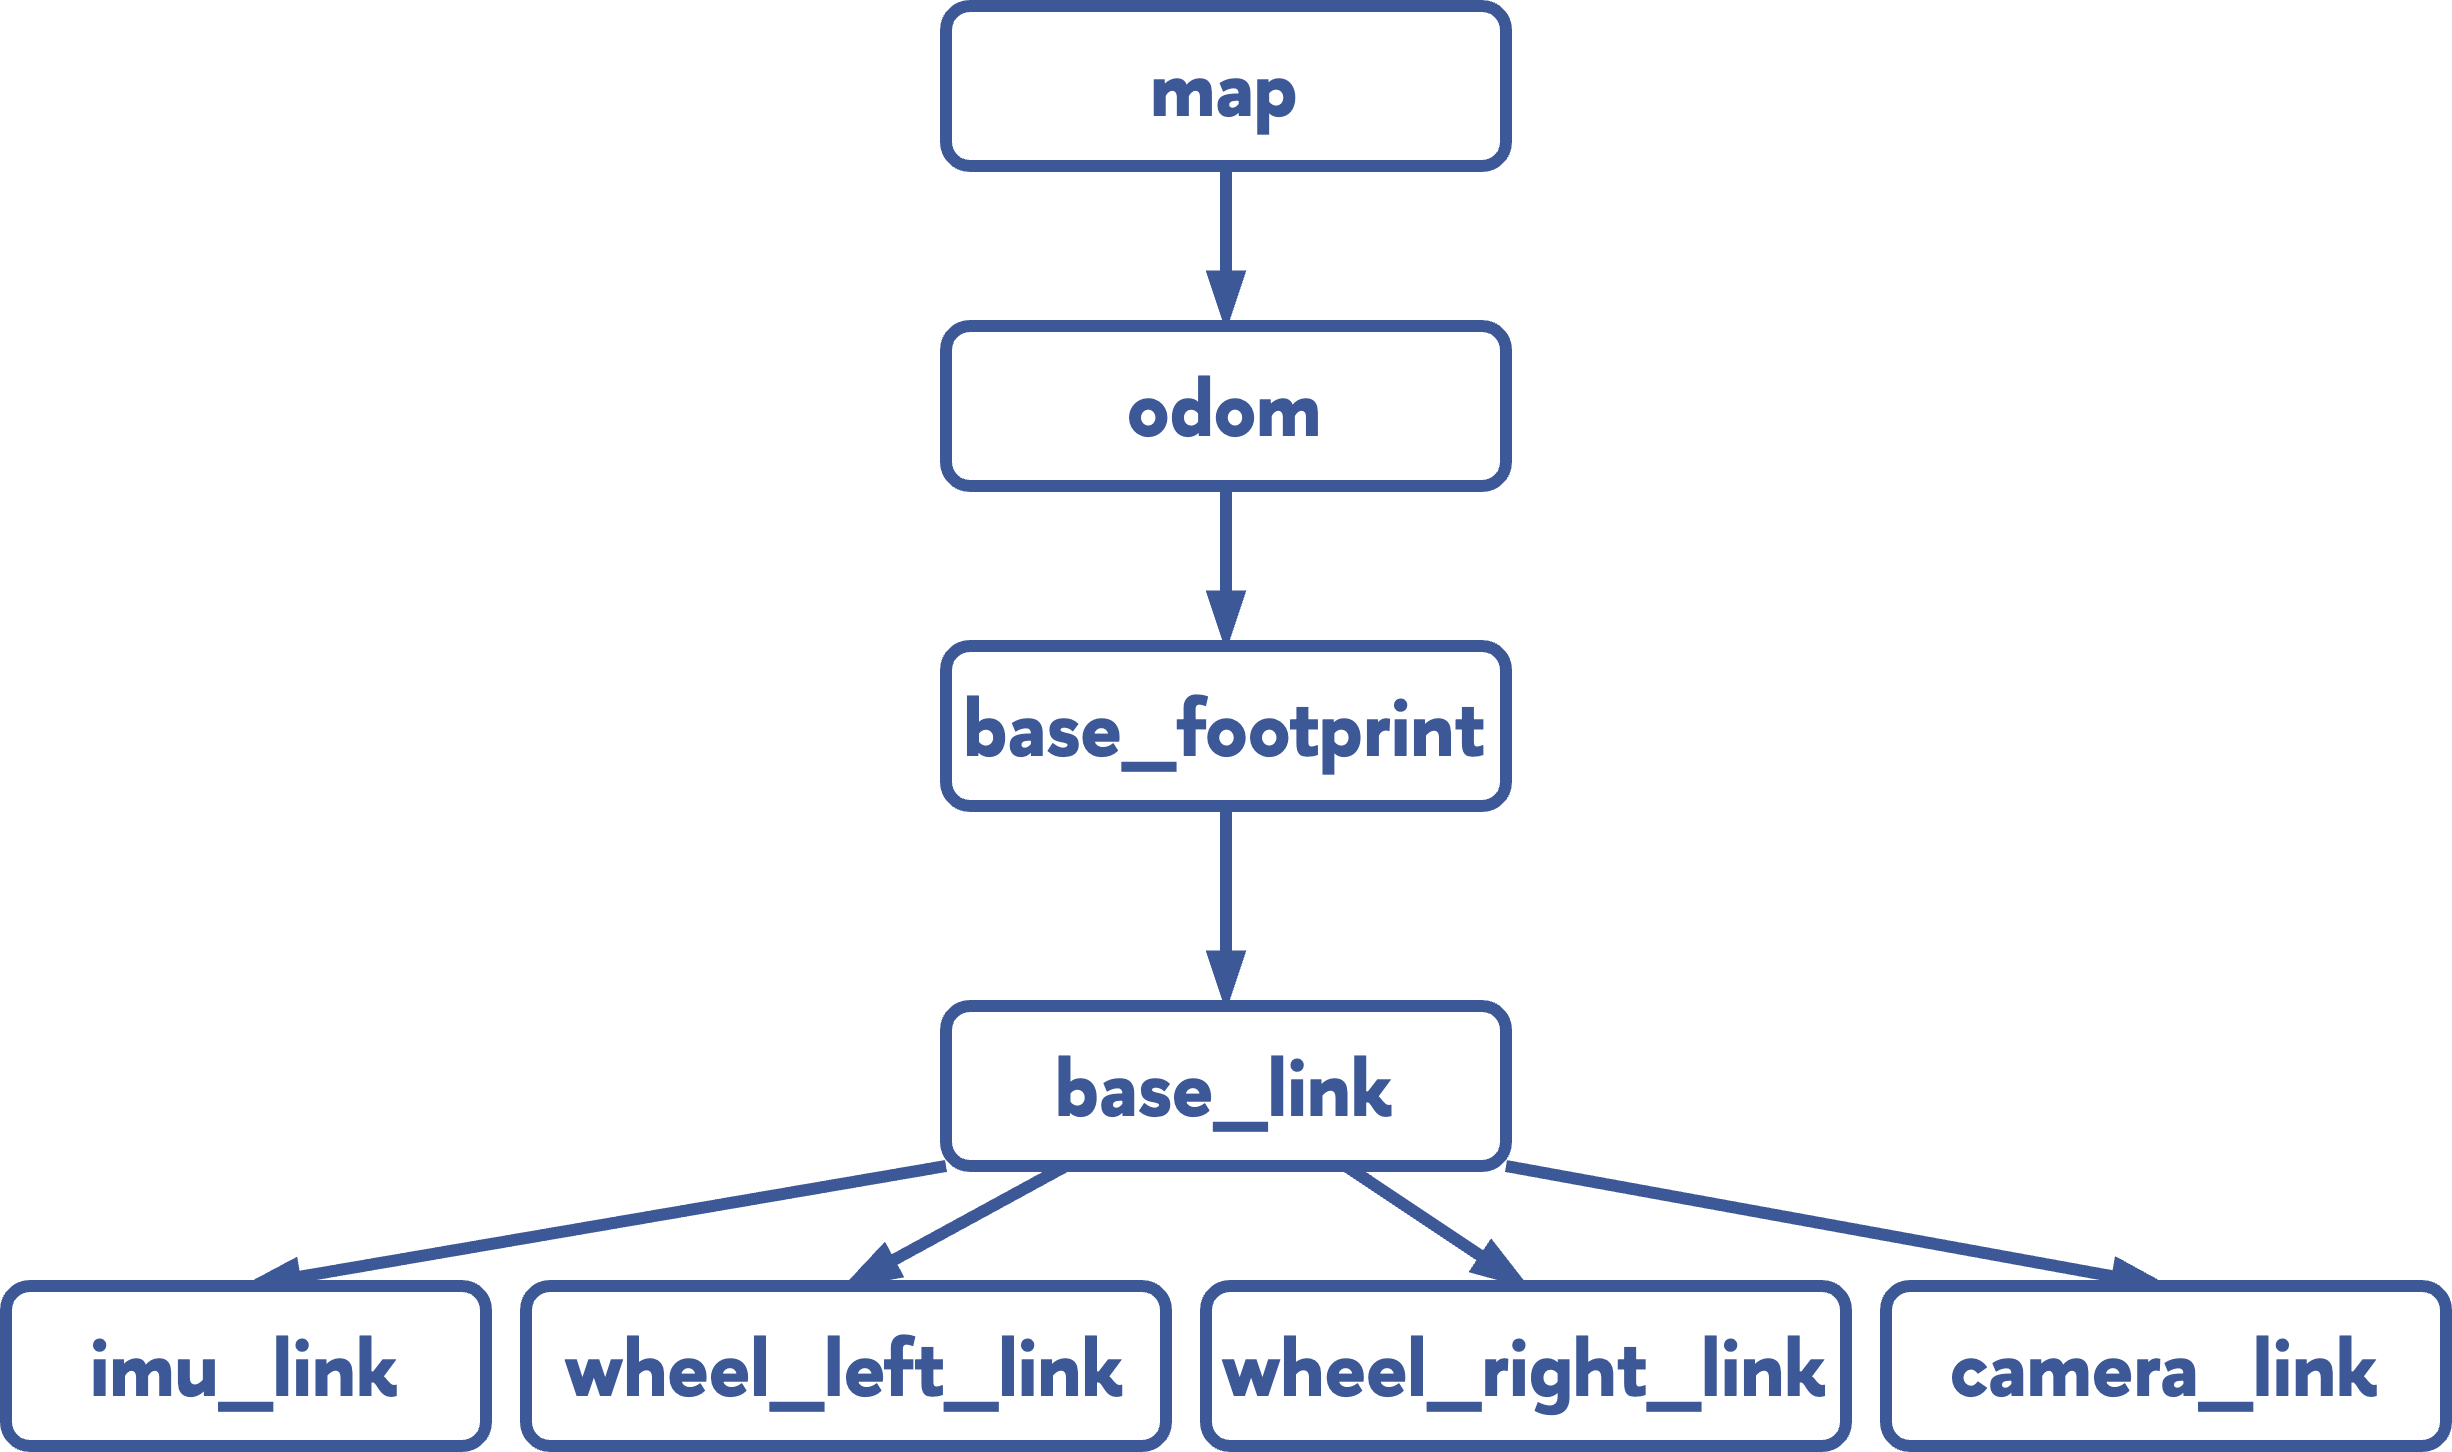
\includegraphics[width=\columnwidth]{images/tree.png}
    \vfill
\end{center}
\end{columns}
\end{frame}


\begin{frame}
\frametitle{Системы координат в ROS2}
\begin{columns}[T]
\column{0.60\textwidth}
\small
\begin{block}{Конвенция имен}
\begin{itemize}
  \item \cmd{base\_link} -- система координат корпуса робота.
  \item \cmd{base\_footprint} --  система координат проекции корпуса на пол.
  \item \cmd{odom} -- система координат точки начала движения.
  \item \cmd{map} -- система координат карты.
  \item Системы координат колес и датчиков — дочерние по отношению к \cmd{base\_link}.
  \item   Одометрия задает \cmd{odom} $\to$ \cmd{base\_link} или \cmd{base\_footprint}, локализация задает \cmd{map} $\to$ \cmd{odom}.
\end{itemize}
\end{block}
\column{0.39\textwidth}
\begin{center}
    \vfill
    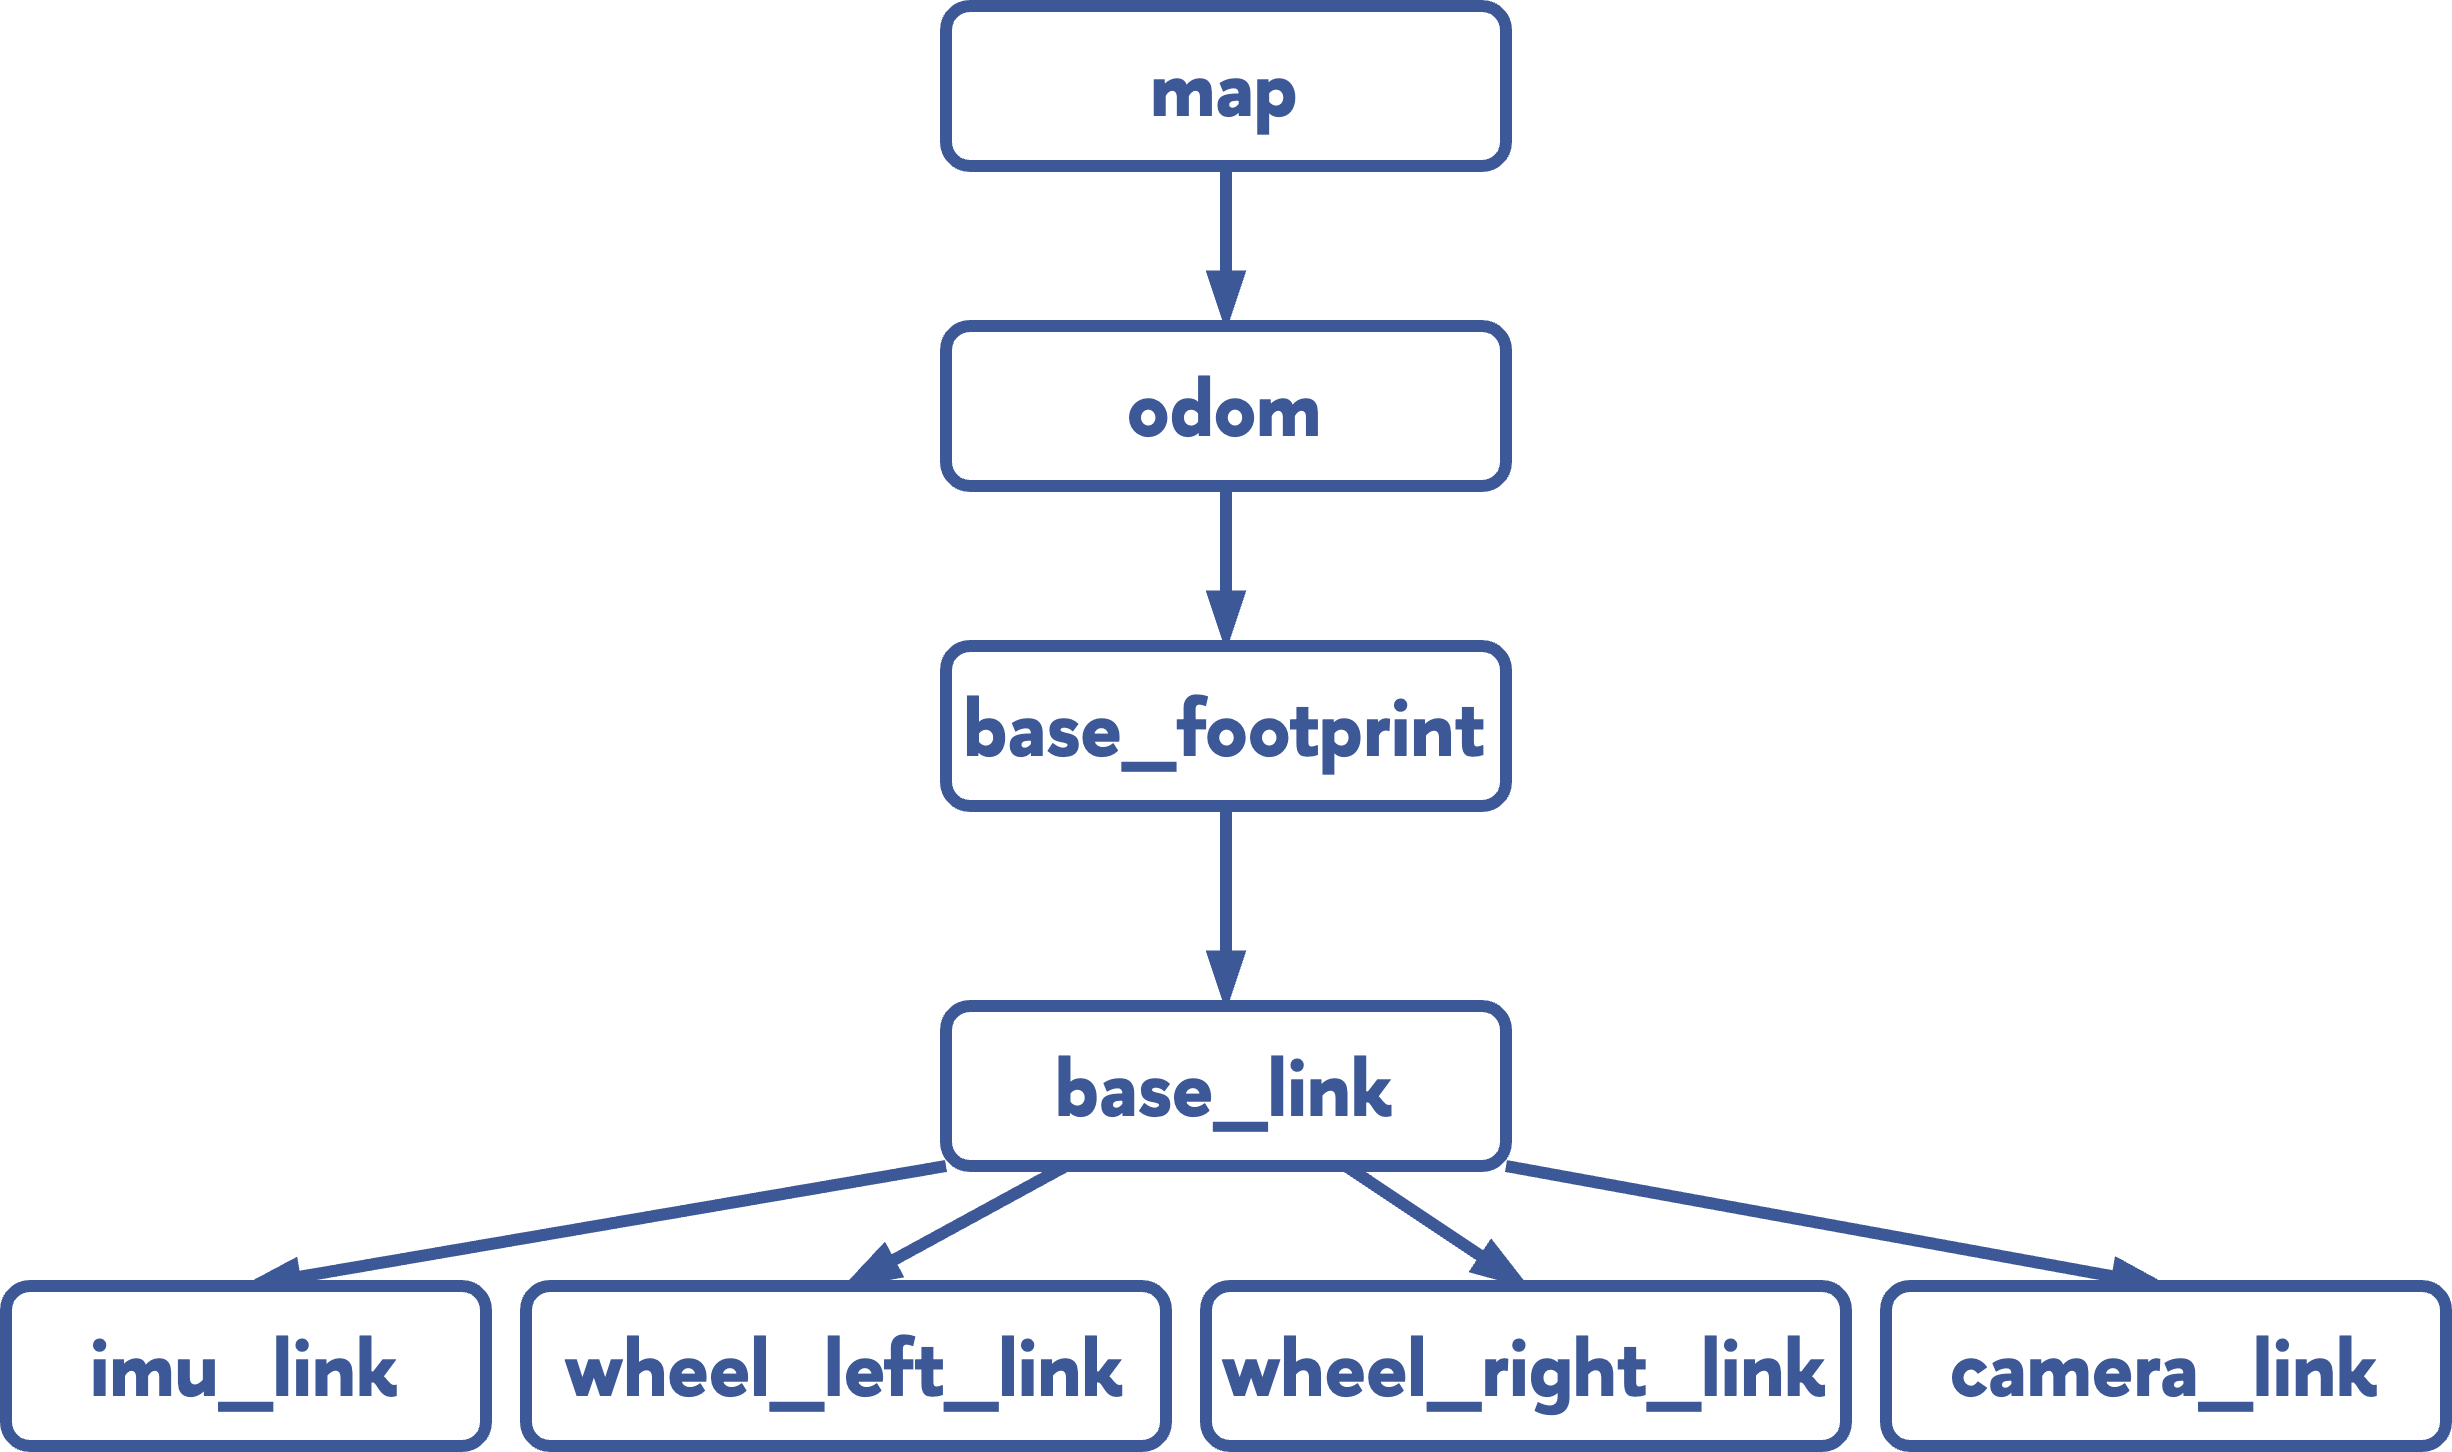
\includegraphics[width=\columnwidth]{images/tree.png}
    \vfill
\end{center}
\end{columns}
\end{frame}

\begin{frame}[fragile]
\frametitle{Системы координат в ROS2}
\small
\begin{itemize}
  \item Передача информации о преобразованиях происходит через публикации в специальных топиках
    \item Преобразования делятся на статические (топик \cmd{/tf\_static}) и динамические  с временными метками (топик \cmd{/tf}).
  \item Объект \cmd{Buffer} хранит преобразования, \cmd{TransformListener} получает, \cmd{TransformBroadcaster} публикует.
  \item Методы \cmd{lookup\_transform} и \cmd{transform} используются для преобразований.
\end{itemize}
\begin{center}
\begin{minipage}{0.8\textwidth}
\begin{lstlisting}[basicstyle=\color{HSEblue}\ttfamily\scriptsize]
from tf2_ros import Buffer, TransformListener
from rclpy.time import Time
import tf2_geometry_msgs
...
self.tf_buffer = Buffer()
self.tf_listener = TransformListener(self.tf_buffer, self)
tf = self.tf_buffer.lookup_transform('base_link', 'laser', Time())
point_base = self.tf_buffer.transform(point, 'base_link')
\end{lstlisting}
\end{minipage}
\end{center}
\end{frame}


\begin{frame}
\frametitle{Управление роботом в ROS2}
\renewcommand{\arraystretch}{1.15}
\small
\begin{tabular}{
  >{\centering\arraybackslash}m{0.05\textwidth}|
  >{\raggedright\arraybackslash}m{0.35\textwidth}
  >{\raggedright\arraybackslash}m{0.55\textwidth}
}
\toprule
\multicolumn{2}{c}{
  Аппаратный интерфейс
}
& Интерфейс взаимодействия с компонентами робота
  или роботом в симуляции \\
\midrule

\multirow{3}{*}{\rotatebox[origin=c]{90}{\cmd{ros2\_control}}}
& \cmd{controller\_manager}
& Управление состоянием контроллеров \\

& \cmd{diff\_drive\_controller}
& Преобразование скоростей корпуса в скорости колес,
  вычисление колесной одометрии \\

& \cmd{joint\_state\_broadcaster}
& Чтение состояния суставов робота из аппаратного интерфейса
  и публикация в топике \cmd{/joint\_states} \\
\midrule

\multicolumn{2}{c}{
  \cmd{robot\_state\_publisher}
}
& Публикация преобразований между компонентами робота
  в \cmd{/tf} и \cmd{/tf\_static}
  на основе \cmd{joint\_states} и описания в специальном формате URDF \\
\bottomrule
\end{tabular}
\end{frame}

\begin{frame}
\frametitle{Управление роботом в ROS2}
\vfill
\begin{center}
\begin{minipage}{0.95\textwidth}
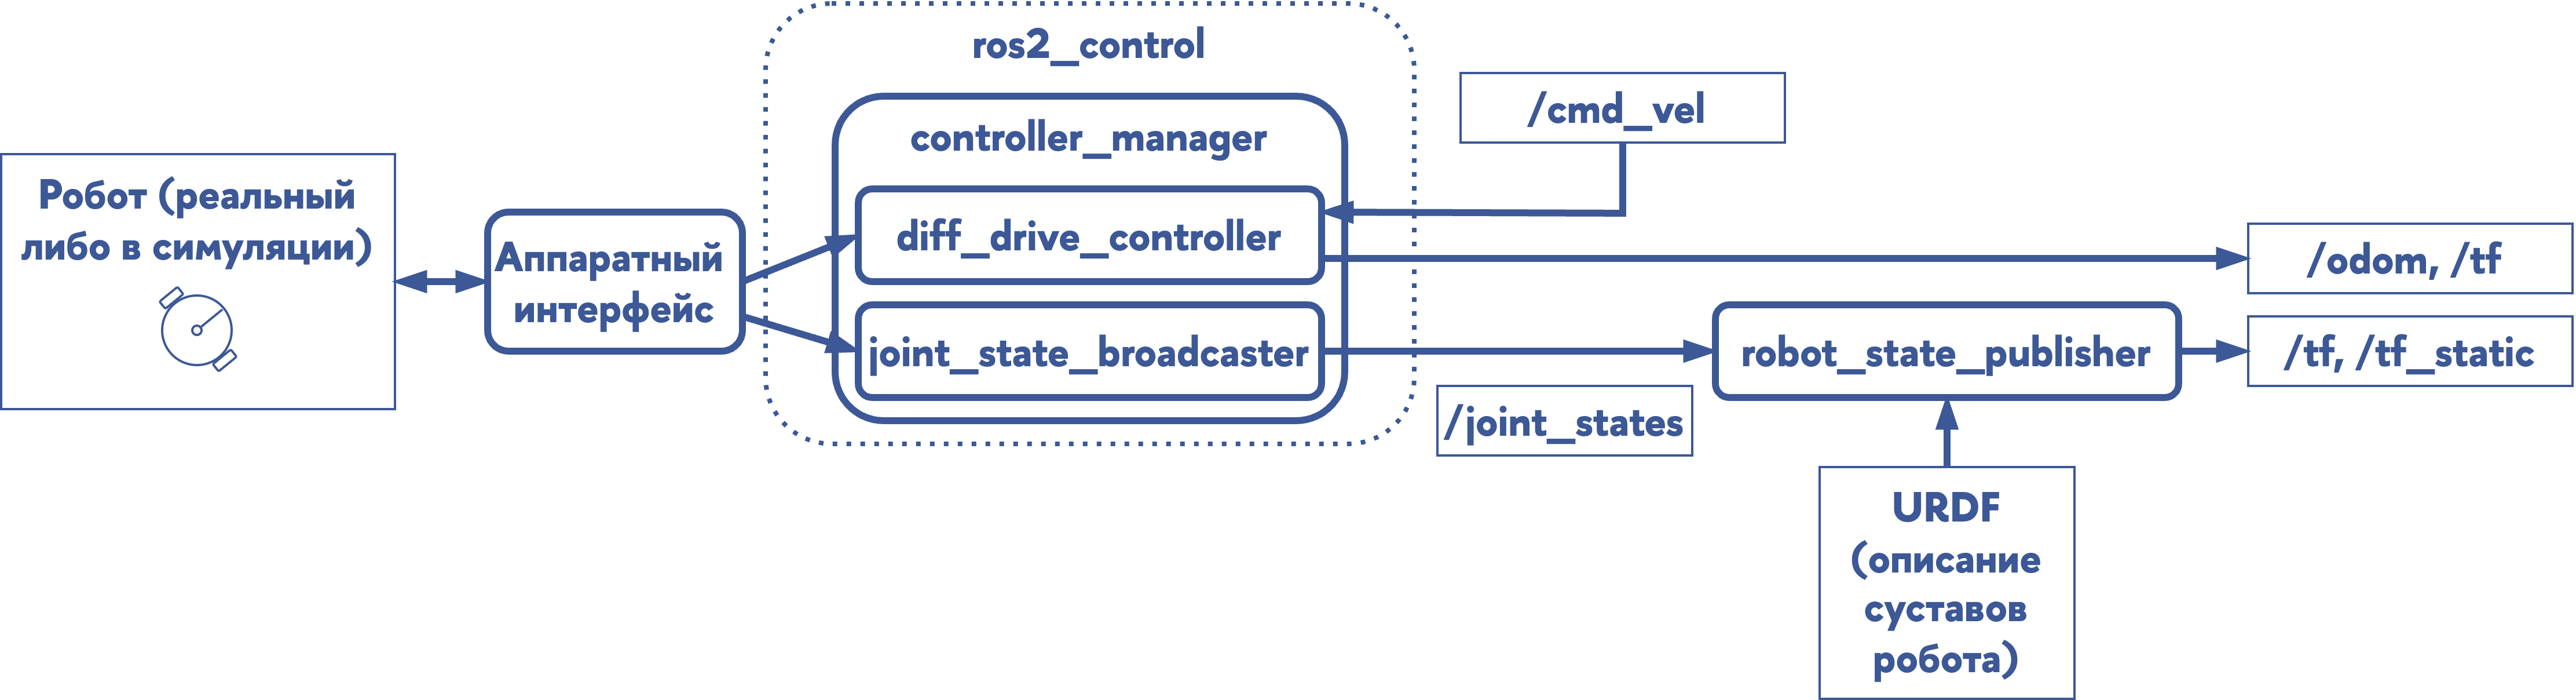
\includegraphics[width=\columnwidth]{images/pipeline.png}
\end{minipage}
\end{center}
\vfill
\end{frame}

\begin{frame}[fragile]
\frametitle{Одометрия в ROS2}
\small
\begin{itemize}
  \item Одометрия публикуется в двух вариантах:

  \item В топике \cmd{/odom} в формате \cmd{nav\_msgs/msg/Odometry}: позиция, скорость и ковариации.
  \item В преобразовании \cmd{odom} $\to$ \cmd{base\_link}: только позиция, без скоростей и ковариаций.
  \item Поза и время должны быть согласованы. У преобразования должен быть один издатель.
\end{itemize}
\vfill
\begin{center}
\begin{minipage}{0.9\textwidth}
\begin{lstlisting}[basicstyle=\color{HSEblue}\ttfamily\footnotesize]
ros2 topic echo /odom
ros2 run tf2_ros tf2_echo odom base_link
\end{lstlisting}
\end{minipage}
\end{center}
\vfill
\end{frame}

\begin{frame}[fragile]
\frametitle{Визуализация и диагностика}
\small
\begin{itemize}
  \item \cmd{tf2\_echo} -- посмотреть отдельное преобразование.
  \item \cmd{tf2\_tools view\_frames} -- дерево преобразований систем координат. 
  \item \cmd{RViz2} -- визуализация модели робота, TF, карты, данных датчиков и др. в 3D.
  \item \cmd{Foxglove} -- 3D-сцена, графики,  просмотр сообщений, просмотр дерева преобразований и многое другое.
\end{itemize}
\vfill
\begin{center}
\begin{minipage}{0.9\textwidth}
\begin{lstlisting}[basicstyle=\color{HSEblue}\ttfamily\footnotesize]
ros2 run tf2_ros tf2_echo odom base_link
ros2 run tf2_tools view_frames
ros2 run rviz2 rviz2
ros2 launch foxglove_bridge foxglove_bridge_launch.xml
\end{lstlisting}
\end{minipage}
\end{center}
\vfill
\end{frame}

\begin{frame}[fragile]
\begin{center}
\Large Спасибо за внимание!
\end{center}
\vfill
\end{frame}

\end{document}
